% fig01_structure_vs_number.tex — standalone TikZ separation diagram.
% Compiled by the paper Makefile via `make figures` (pdflatex on the snippet,
% no Python/external dep). In main.tex \includegraphics the COMPILED pdf —
% do NOT \input this .tex.
%
% Two axes:
%   x = axis assignment (structure on left, number on right)
%   y = verdict outcome (SUPPORTED top, FALSIFIED bottom)
% Pre-registered claim: all 8 H land on the diagonal SUPP/structure (top-left)
% or FAL/number (bottom-right) cells. No point in the off-diagonal cells.
\documentclass[tikz,border=6pt]{standalone}
\usepackage{pgfplots}
\pgfplotsset{compat=1.18}
\begin{document}
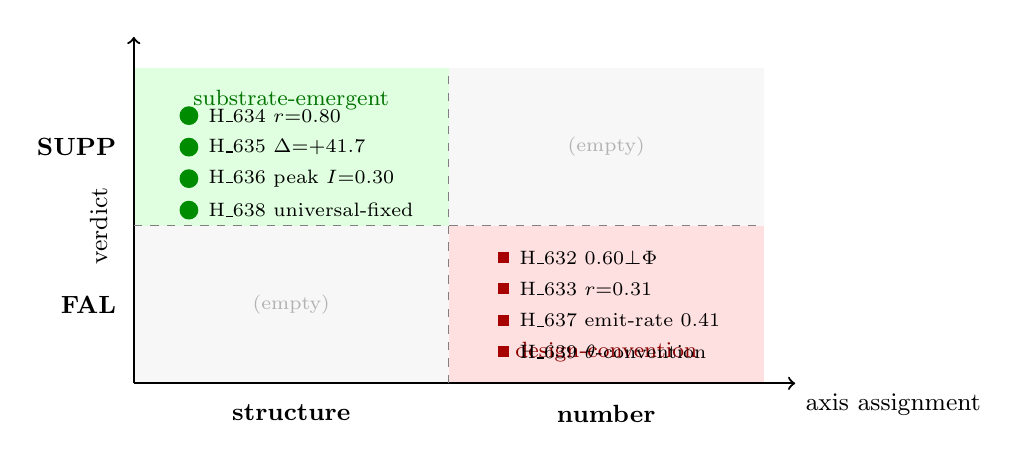
\begin{tikzpicture}
  % quadrant background: emergent (top-left) green, convention (bottom-right) red
  \fill[green!12]  (0,2.0) rectangle (4,4);     % structure x SUPP
  \fill[red!12]    (4,0)   rectangle (8,2.0);    % number    x FAL
  \fill[gray!6]    (4,2.0) rectangle (8,4);      % off-diag (empty)
  \fill[gray!6]    (0,0)   rectangle (4,2.0);    % off-diag (empty)

  % axes
  \draw[->,thick] (0,0) -- (8.4,0) node[below right]{\small axis assignment};
  \draw[->,thick] (0,0) -- (0,4.4) node[above left,rotate=90,anchor=south]{};
  \node[rotate=90] at (-0.45,2) {\small verdict};
  \draw[dashed,gray] (4,0) -- (4,4);
  \draw[dashed,gray] (0,2.0) -- (8,2.0);

  % axis ticks
  \node[below] at (2,-0.15) {\small\textbf{structure}};
  \node[below] at (6,-0.15) {\small\textbf{number}};
  \node[left]  at (-0.1,3.0) {\small\textbf{SUPP}};
  \node[left]  at (-0.1,1.0) {\small\textbf{FAL}};

  % quadrant labels
  \node[green!45!black] at (2,3.6) {\footnotesize substrate-emergent};
  \node[red!55!black]   at (6,0.4) {\footnotesize design-convention};

  % structure x SUPP (4 green points, top-left)
  \node[circle,fill=green!55!black,inner sep=2.4pt,label=right:{\scriptsize H\_634 $r{=}0.80$}] at (0.7,3.4) {};
  \node[circle,fill=green!55!black,inner sep=2.4pt,label=right:{\scriptsize H\_635 $\Delta{=}{+}41.7$}] at (0.7,3.0) {};
  \node[circle,fill=green!55!black,inner sep=2.4pt,label=right:{\scriptsize H\_636 peak $I{=}0.30$}] at (0.7,2.6) {};
  \node[circle,fill=green!55!black,inner sep=2.4pt,label=right:{\scriptsize H\_638 universal-fixed}] at (0.7,2.2) {};

  % number x FAL (4 red points, bottom-right)
  \node[rectangle,fill=red!65!black,inner sep=2.0pt,label=right:{\scriptsize H\_632 $0.60{\perp}\Phi$}] at (4.7,1.6) {};
  \node[rectangle,fill=red!65!black,inner sep=2.0pt,label=right:{\scriptsize H\_633 $r{=}0.31$}] at (4.7,1.2) {};
  \node[rectangle,fill=red!65!black,inner sep=2.0pt,label=right:{\scriptsize H\_637 emit-rate $0.41$}] at (4.7,0.8) {};
  \node[rectangle,fill=red!65!black,inner sep=2.0pt,label=right:{\scriptsize H\_639 $\theta$-convention}] at (4.7,0.4) {};

  % off-diagonal: explicitly empty
  \node[gray!60] at (6,3.0) {\scriptsize (empty)};
  \node[gray!60] at (2,1.0) {\scriptsize (empty)};
\end{tikzpicture}
\end{document}
